% Straight up stealing preamble from Eli Holmes 
%%%%%%%%%%%%%%%%%%%%%%%%%%%%%%%%%%%%%%START PREAMBLE THAT IS THE SAME FOR ALL EXAMPLES
\documentclass{article}

%Required: You must have these
\usepackage{Sweave}
\usepackage{graphicx}
\usepackage{tabularx}
\usepackage{hyperref}
\usepackage{natbib}
\usepackage{pdflscape}
\usepackage{array}
\usepackage{gensymb}
%\usepackage[backend=bibtex]{biblatex}
%Strongly recommended
 %put your figures in one place
 
%you'll want these for pretty captioning
\usepackage[small]{caption}

\setkeys{Gin}{width=0.8\textwidth} %make the figs 50 perc textwidth
\setlength{\captionmargin}{30pt}
\setlength{\abovecaptionskip}{0pt}
\setlength{\belowcaptionskip}{10pt}
% manual for caption http://www.dd.chalmers.se/latex/Docs/PDF/caption.pdf

%Optional: I like to muck with my margins and spacing in ways that LaTeX frowns on
%Here's how to do that
 \topmargin -2cm     
 \oddsidemargin -0.04cm   
 \evensidemargin -0.04cm  % same as oddsidemargin but for left-hand pages
 \textwidth 16.59cm
 \textheight 22.94cm 
 %\pagestyle{empty}       % Uncomment if don't want page numbers
 \parskip 7.2pt           % sets spacing between paragraphs
 %\renewcommand{\baselinestretch}{1.5} 	% Uncomment for 1.5 spacing between lines
\parindent 0pt% sets leading space for paragraphs
\usepackage{setspace}
%\doublespacing

%Optional: I like fancy headers
\usepackage{fancyhdr}
\pagestyle{fancy}
\fancyhead[LO]{Do early phenological events constrain later phenology?}
\fancyhead[RO]{2017}
 
%%%%%%%%%%%%%%%%%%%%%%%%%%%%%%%%%%%%%%END PREAMBLE THAT IS THE SAME FOR ALL EXAMPLES

%Start of the document
\begin{document}

% \SweaveOpts{concordance=TRUE}
\bibliographystyle{/Users/aileneettinger/citations/Bibtex/styles/amnat.bst}
\title{Do early phenological events constrain later phenology?} 
\author{A.K. Ettinger, S. Gee, and E.M. Wolkovich}
%\date{\today}
\maketitle  %put the fancy title on
%\tableofcontents      %add a table of contents
%\clearpage
%%%%%%%%%%%%%%%%%%%%%%%%%%%%%%%%%%%%%%%%%%%%%%%%%%%

%We plan to submit this paper as a ``brief communication' at American Journal of Botany (``short (3000-5000 word) research articles reporting exciting, significant new findings. They include no more than 4 figures and tables, combined. Manuscripts, and their abstracts, should be organized as described for Research articles.") or a ``rapid report" at New Phytologist.

\section*{Abstract}
\subsection*{Premise of the study}
We test the extent to which previous phenological stages constrain later ones, throughout a growing season and across 25 angiosperm tree species. 
\subsection*{Methods}
\subsection*{Key results}
\subsection*{Conclusions}
\section* {Key words}
plant phenology, climate change, bud-burst, leaf-out, angiosperm, tree
\section* {Introduction}
Plant phenology, the timing of life-events such as leaf-out and flowering, is a critical trait that affects individual fitness, population abundance, agricultural and natural productivity, and global climate, through its role in carbon sequestration \citep{miller-rushing2008,primack2009a,willis2010,miller-rushing2010}. In temperate tree species, temperature is thought to be a major factor controlling phenology \citep{parmesan2006, morin2010,schwartz2013}. As such, recently observed temporal shifts in bud-burst, leaf-out, and other phenological states have been attributed to warming from anthropogenic climate change\citep{parmesan2006}. Phenology is expected to shift further with future climate change, and, because of its important role in many ecosystem services and in the global climate cycle, planning and preparing for climate change impacts will benefit from improved understanding and forecasting of tree phenology.
\par Despite the observation that spring phenology generally shifts earlier with warmer temperatures, dramatic variation exists in phenological responses to climate. Different tree species vary widely in the timing of leaf-out and other phenological processes, even when exposed to the same environmental conditions \citep{lechowicz1984,primack2009c}. For example, spring lea-out can span weeks among coexisting tree species \citep{lechowicz1984}. The drivers of these variations are poorly understood, even though phenology has been long-observed \citep{wolkovich2014}.
\par One important feature of plant phenology is that events are sequential: leaf bud-burst comes before leaf-out, flowering comes before fruiting, etc. This ordering may constrain phenological events, but the extent of constraints between phenological events is poorly understood because few studies have integrated across consequtive events. Here, we examine the extent to which previous phenological events constrain later events. Specifically, we test two hypotheses:
\begin{itemize}
\item Hypothesis 1: Previous phenological events constrain later events; e.g., late-fruiting species set fruit late in the season because they leaf-out late  (Figure \ref{fig:hyp}).
\item Hypothesis 2: Inter-phenophase time  constrains phenology; e.g., late-fruiting species set fruit late in the season because they require longer maturation time (Figure \ref{fig:hyp}).
\end{itemize}

\section* {Materials and Methods}
\subsection*{Study site and focal species}
This study was conducted at the Arnold Arboretum of Harvard University, a 281-acre park in Boston, Massachusetts, established in 1872. It contains a living collection of 3,825 woody plant taxa that are native to North America, Europe, and Asia. Arboreta are great resources for phenological studies across many species \citep{primack2009a}, particularly in temperate areas, since they may contain a higher diversity of tree species growing in one location than nearby natural areas. In addition, there is often high variation in phenology in the species planted in arboreta, for public enjoyment. For this study, we selected 25 focal angiosperm species that varied in their flowering times (Table 1). We selected up to five individuals of each species for the study, yielding a total of 118 individuals.

\subsection*{Phenology data collection}
Phenology was quantified following the National Phenology Network (NPN) protocols \citep{denny2014}. The bud-burst phase is characterized by green leaf tips being visible at the tips of buds. The leaf-out phase is characterized by visible fully unfolded leaves and petioles that have completely emerged from the buds. Leaf senescence is characterized by leaves changing from green to fall colors. The flowering phase is when open flowers are visible, and the fruiting phase is when developing fruit are visible. 
\par We visited each individual once every 6-10 days throughout the growing season. Phenology observations in the spring began on April 6, 2015, and fall phenology observations ended on December 2, 2015.
From the phenology data, we extracted the day of the year (DOY) of the first observed occurrence of a given phenological phase. Bud-burst DOY was defined as the first day when three or more leaf buds were seen bursting. Leaf-out DOY was defined as the first day when 5\% or more of the individual was leafing out. Flowering DOY was defined as the first day when 5\% or more of the flower buds were open on an individual. Fruiting DOY was defined as the first day when three or more developing fruits were observed on the individual. Leaf senescence DOY was defined as the first day when 5\% or more of the individual showed fall colors \citep{denny2014}.
\subsection*{Statistical analyses}
To understand the extent to which previous phenological events constrain later events (Hypothesis 1, Figure \ref{fig:hyp}), we fit linear models in which the response variable was phenological stage (i.e. the species-level mean day of year of leaf-out, flowering, fruiting, or senescence; bud-burst, the earliest stage we quantified, was excluded), and the predictor was previous phenologival stage.  We therefore fit 10 different models, each with one of the previous phenological stages as the predictor variable. 
All analyses were conducted in R version 3.2.4 \citep{rcoreteam2016}.

\section* {Results}
\par We monitored five phenophases, which varied in duration. Bud-burst occurred over 32 days in the spring, and leaf-out occurred over 30 days, across all focal species \ref{fig:focsp}. Flowering phenology occurred over a longer period than bud-burst and leaf-out, spanning 111 days from late April to September \ref{fig:focsp}. Fruiting spanned 183 days, and leaf senescence occurred over 56 days\ref{fig:focsp}. %I took these numbers from Sally's thesis, but i'm actually not sure how she got them...they don't seem to match the average numbers that appear in ref{fig:focsp}
Most species (20/25) spent the majority of the growing season in the reproductive phenological phases (i.e. flowering and fruit development), and most species (23/25) began leaf bud-burst prior to flowering, though leaf development overlapped with flowering in some species \ref{fig:focsp}.
\par We found strong correlations between late versus early phenology stages in many cases (Figures \ref{fig:focsp}, \ref{fig:latevearly}), suggesting that earlier phenological stages constrain later ones. The strongest correlations occurred between adjacent stages (i.e. those along the diagonal in Figure \ref{fig:latevearly}, such as leaf-out and bud-burst, fruiting and flowering). Senescence was the only phenological stage not well-correlated with an earlier phanological stage.
\par We also observed strong correlations between phenology and inter-phenophase duration for bud-burst and for both reproductive pheno-phases stages (flowering and fruiting time, Figure \ref{fig:inter}). Reproductive phenology appears to be constrained by both earlier inter-phenophase times (e.g. flowering DOY was correlated with days between flowering and bud-burst, fruiting DOY is correlated with days between fruiting and flowering stages) and later interphase times (e.g. flowering DOY was correlated with days between senescence and flowering). Bud-burst day of year, which was the earliest phenophase we observed in the growing season, was most strongly related to inter-phenophase time between leaf-out and bud-burst. For other growth phenophases (leaf-out, senescence), inter-phenophase time was not a strong predictor of phenology (Figure \ref{fig:inter}). 

\section* {Discussion}
\par The majority of phenological stages we observed (three out of four) support Hypothesis 1: their timing appears to be constrained by earlier phenological stages.  Add rate of change (effect size) for different models. Thus, environmental conditions in the winter or spring that may directly only affect early phenologial stages, such as bud-burst, are likely to have cascading effects on later stages such as leaf-out, flowering, and fruiting. 
\par Reproductive phenology (flowering and fruiting) also supported Hypothesis 2: timing appears to be constrained by inter-phenophase time. Later flowering species require more time between flowering and budburst.%(with flowering time delayed 1.03 days per day of inter-phenophase time) 
and betwee flowering and leaf-out. %(with flowering time delayed 1.10 days per day of inter-phenophase time)
Similarly, late fruiting species had longer inter-phenophase time between between fruiting and flowering.%(with fruiting time delayed 1.11 days per day of inter-phenophase time). 
These results are consistent with previous theories that trees investing more resources into their offspring (i.e. having larger seeds) flower and fruit earlier because they need more time to build resources for the offspring (Bolmgren and Cowan, 2008; Sun and Frelich, 2011).
\par Our findings highlight that our two hypotheses are not mutually exclusive. For example, we found a positive relationship between bud-burst and leaf-out ( Figure \ref{fig:latevearly}). However, earlier bud-burst does not always result in earlier leaf-out; for some species, it is associated with longer time between bud-burst and leaf-out (Figure \ref{fig:inter}). From our one year of data, it is not clear if this pattern is due to variation in species' physiology and drivers of phenology, or to weather patterns. For example, many species leafed out after DOY 130 (May 10, 2015), despite bud-burst days ranging from day 110 to 130. Its possible that, after a cold and wet spring, warming occurred suddenly around May 10, 2015. 
  
%Ended up not having much to say about this point, so cut the below paragraph, but Lizzie, if you think this should be included, please add some notes or ideas:
%\par Perhaps expect correlations could be strongest at biggest at end of season(senesence)? Geometric constraint. Also, perhaps relevant, from Sally's thesis: "Leaf senescence is less studied and more poorly understood, compared to spring phenological phases (Parmesan, 2006). However, it is important that future studies focus on understanding this phenological phase, since it can drive changes in growing season length (Jeong et al., 2011), and since climate change is linked to the phenomenon of later fall (Richardson et al. 2006; Jeong et al., 2011)."
\par There are atleast two important implications of these findings for improved forecasting of climate change induced shifts in phenology. First, a shift in one phase may have cascading effects on later phases, since each phase is linked to phases that occur before and after it \citep{wolkovich2014b}. This highlights a clear need to conduct future studies across entire growing seasons, at a minimum    \citep{wolkovich2014}, and begs the question of how phenophases may be linked across years, as well. We wonder, for instance, whether the timing of spring bud-burst in one year may be related to the timing of bud-set the previous fall (add citations?). Second, given the species-specific nature of phenological constraints, accurate forecasts of community-wide phenological shifts are likely to require species-specific information, such as fruit development time for fruiting forecasts, in addition to climate data \citep{diez2012}. %Not sure about the Second implication here....maybe it should just be one implication and focus on the first one?

\section* {Conclusions}
Many questions remain about drivers of the dramatic variation observed to date in phenological patterns and shifts in these patterns under anthropogenic climate change. Given our findings that consecutive stages are linked, we encourage future studies, whether observational or manipulative, to collect data across entire growing seasons. Multi-year studies will be critical to evaluate the extent to which the phenological patterns are consistent among years that may vary in climate, as well as biotic conditions (i.e. pollinator or pest populations).  % Other things to add: Encourage a phylogenetic approach, collect data across years. We observed variation at whole organism level- may want to explore at individual flower/fruit level. 
Improved understanding of phenological constraints and drivers of phenological variation offers the potential for improved forecasts of phenological shifts  with climate change to help predict how ecosystem functions will be altered  in the future.



\section*{Acknowledgements}
We thank H. Eyster, D. Flynn, E. Forrestel, S. Golumbeanu, W. Friedman, R. Mcnellis, J. Samaha, J. Savage, and T. Savas for field and laboratory assistance and advice. We thank J. DelRosso, M. Dosmann, A. Gapinski, K. Richardson, F. Rosin, and the many other curatorial, horticultural, and research staff of the Arnold Arboretum who made this work possible. Research was supported by the Harvard College Research Program (to S.G.), the Grants-In-Aid of Undergraduate Research program of the Museum of Comparative Zoology, the Harvard University Herbaria, and the Arnold Arboretum of Harvard University (to S.G.), and the National Science Foundation (NSF DBI 14-01854 to A.E.). Any opinion, findings, and conclusions or recommendations expressed in this material are those of the authors and do not necessarily reflect the views of the National Science Foundation.

\section*{Data Accessibility}
The dataset for this study is available online at KNB (Cite). 

\section*{Author contributions} All authors conceived and designed the study and edited the manuscript; S.G. conducted the field and lab work; S.G. and A.E. analyzed the data and wrote the manuscript; E.W. edited the manuscript.

\section{Bibliography}
\bibliography{/Users/aileneettinger/citations/Bibtex/mylibrary}

\section* {Tables}

\begin{table}[p]
  \caption{\textbf{Focal species.} Twenty-five angiosperm species were selected, based on their flowering phenology in long-term records of the Arnold Arboretum. (The flowering patterns we observed during our one year of data collection did not always perfectly match these long-term patterns.) The number of individuals of each species observed at the Arnold Arboretum from spring through fall 2015 is in parentheses.}
\begin{footnotesize} 
   \begin{tabular}{| p{5.5cm} | p{5.5cm} | p{5.5cm} |}
    \hline
  \bf{Early season flowering} & \bf{Mid season flowering} & \bf{Late season flowering} \\ \hline
    \textit{Aesculus flava} (5) & \textit{Carya glabra} (5) & \textit{Catalpa speciosa} (5) \\ 
    \textit{Betula alleghaniensis} (5) & \textit{Carya ovata} (5) & \textit{Kalopanax septemlobus} (3) \\ 
    \textit{Betula nigra} (5) & \textit{Crataegus crus-galli} (5) & \textit{Styphnolobium japonicum} (5) \\ 
\textit{Gleditsia triancanthos} (5) & \textit{Fagus engleriana} (4) & \textit{Tilia americana} (5) \\ 
\textit{Liriodendron tulipifera} (5) & \textit{Fagus grandifolia} (5) & \textit{Tilia japonica} (5) \\ 
\textit{Phellodendron amurense} var. \textit{lavallei} (4) & \textit{Fraxinus chinensis} (5) &\\ \textit{Populus deltoids} ssp. \textit{deltoids} (5) & \textit{Liquidambar styraciflua} (5) & \\ 
\textit{Pyrus calleryana} var. \textit{dimorphophylla} (3) & \textit{Platanus occidentalis} (5) & \\ 
\textit{Pyrus ussuriensis} var. \textit{hondoensis} (5) & \textit{Quercus glandulifera} (4) & \\ \textit{Quercus alba} (5) & \textit{Quercus rubra} (5) &  \\ \hline
     \end{tabular}    
\end{footnotesize} 
    \end{table}
\clearpage

\section* {Figures}
\begin{figure}[p]
  \centering
  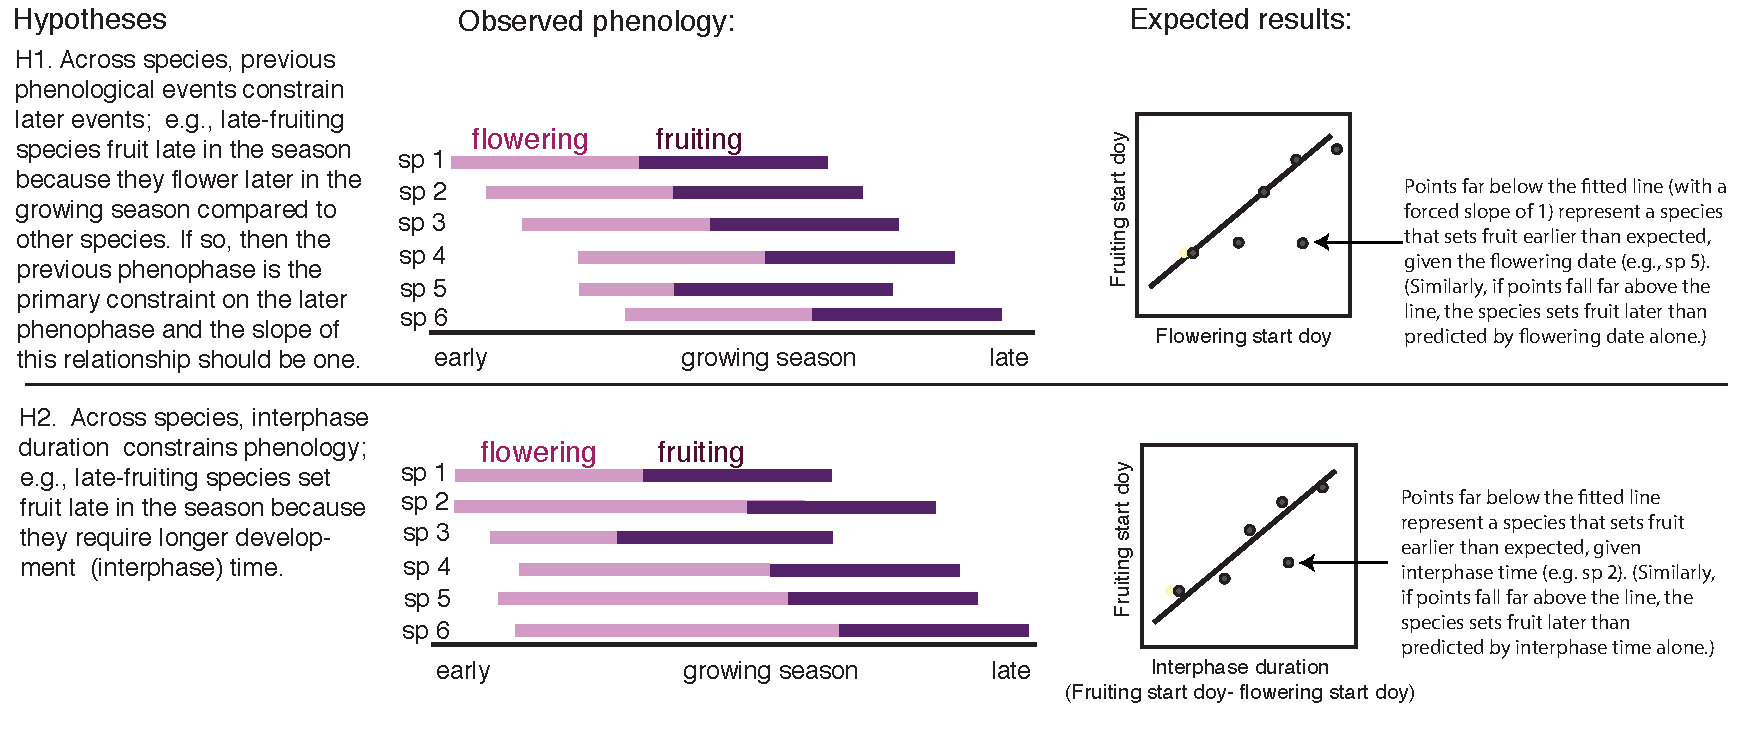
\includegraphics{../analyses/figures/hypotheses3.pdf} 
  \caption{\textbf{Hypotheses.} We show flowering and fruiting as examples of consecutive phenological events. We expected the same patterns for other consecutive events,such as leaf bud-burst and leaf-out. Inter-phenophase duration is the time between phenological events, e.g., the number of days between the start of flowering and the start of fruiting.} 
 \label{fig:hyp}
\end{figure}
 
\begin{figure}[h]
  \centering
  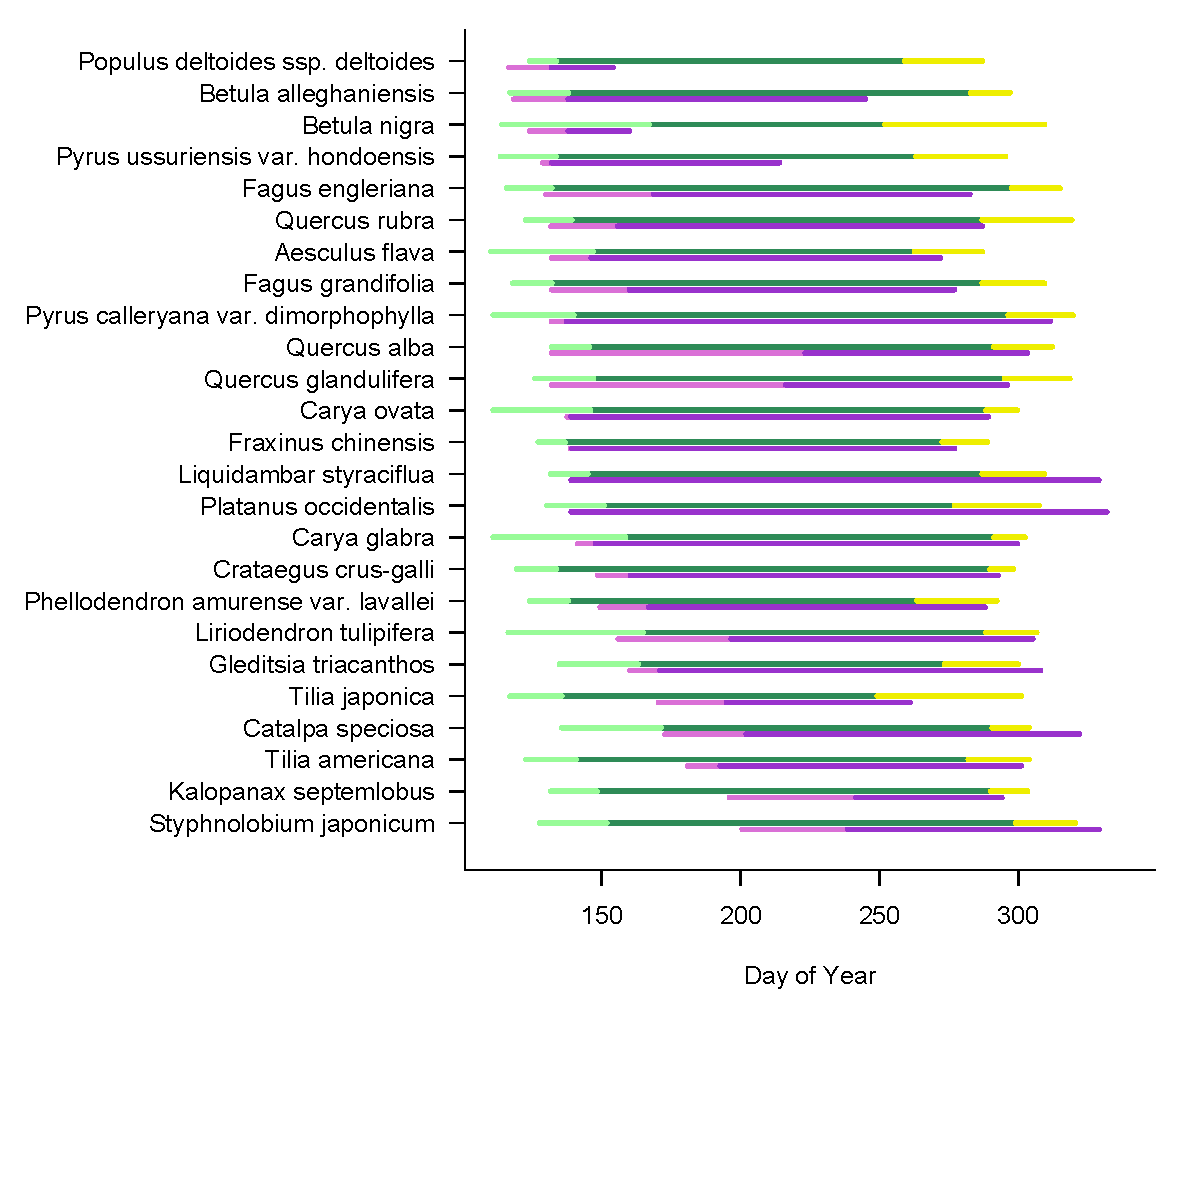
\includegraphics{../analyses/figures/grosea_repsort.pdf}
  \caption{\textbf{Focal species' phenology during the 2015 growing season, sorted by their mean first-flower dates.} For growth phenology, light green represents the bud-burst phase (from its mean start day-of-year to the mean start day-of-year for leaf-out, across all individuals within a species), dark green represents full leaf-out (from the mean day-of-year when fully-expanded leaves were first observed through the start of senescence), and yellow represents the senescence phase (from the mean day-of-year when leaves first began changing color through the mean day-of-year when more than 95 percent of leaves on the tree had changed color). For reproductive phenology, light purple represents the flowering phase (from the mean day-of-year when flowers first appeared to the mean day-of-year when fruits first appeared, across all individuals within a species) and dark purple represents the fruiting phase (from the mean day-of-year when fruits first appeared to the mean day-of-year when more than 95 percent of fruits were first observed as ripe).}
  \label{fig:focsp}
\end{figure}
  
  \begin{figure}[h]
  \centering
  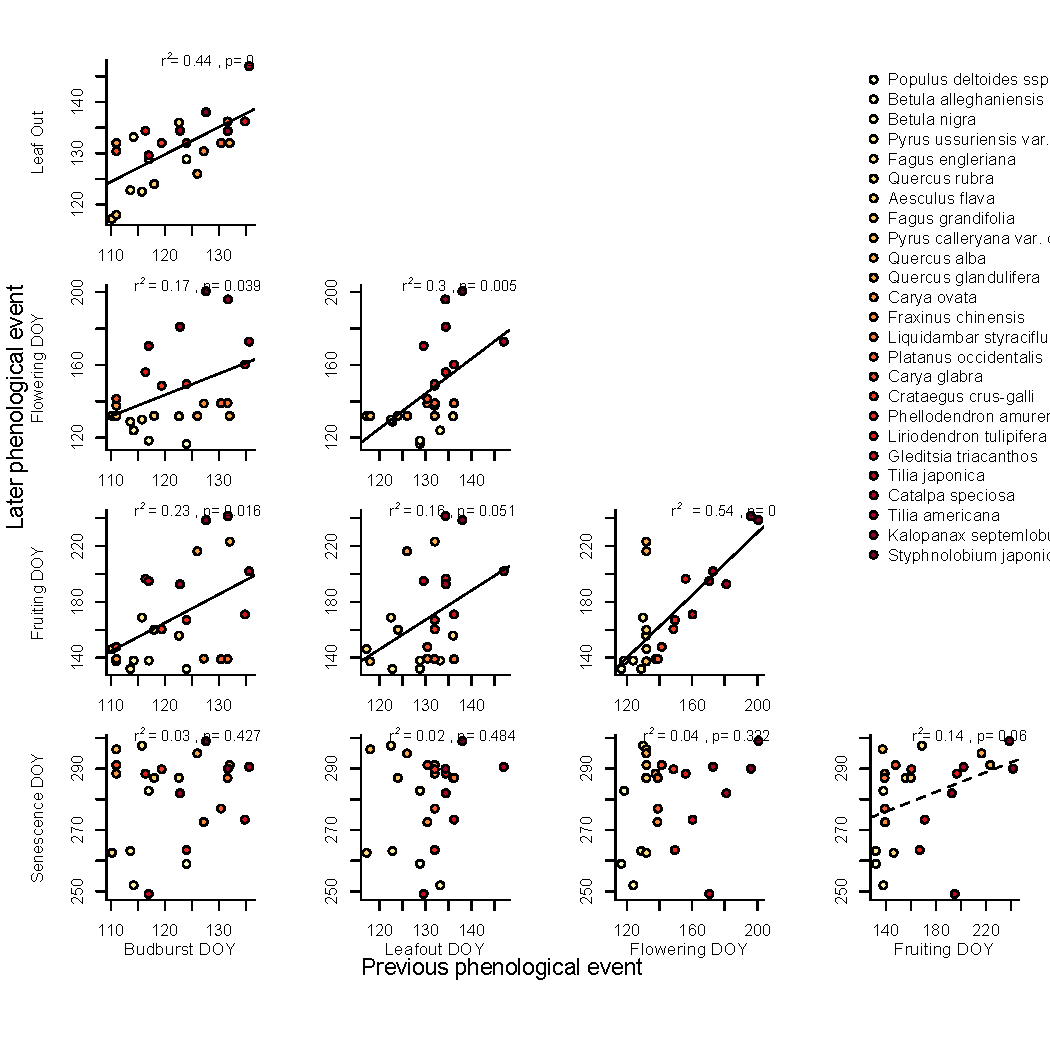
\includegraphics{../analyses/figures/latevearly_rp_col_legend_YOR.pdf}
  
  \caption{\textbf{Relationships among phenological stages across the 25 focal species.} Linear models were fit with the species-level mean day of year of the later phenological stages as the response variable, and mean day of year of earlier stage as the explanatory variable. R\textsuperscript{2} and \textit{p}-value for each model are shown, with solid lines representing model fit when \textit{p}<0.05 and dashed lines representing model fit when 0.05<\textit{p}<0.10. Full model statistics are summarized in Table S1 in the Supplemental Materials. Species in the legend are ordered from early to late first-flower dates, as in Figure 2.}
  \label{fig:latevearly}
\end{figure}
\begin{figure}[h]
  \centering
  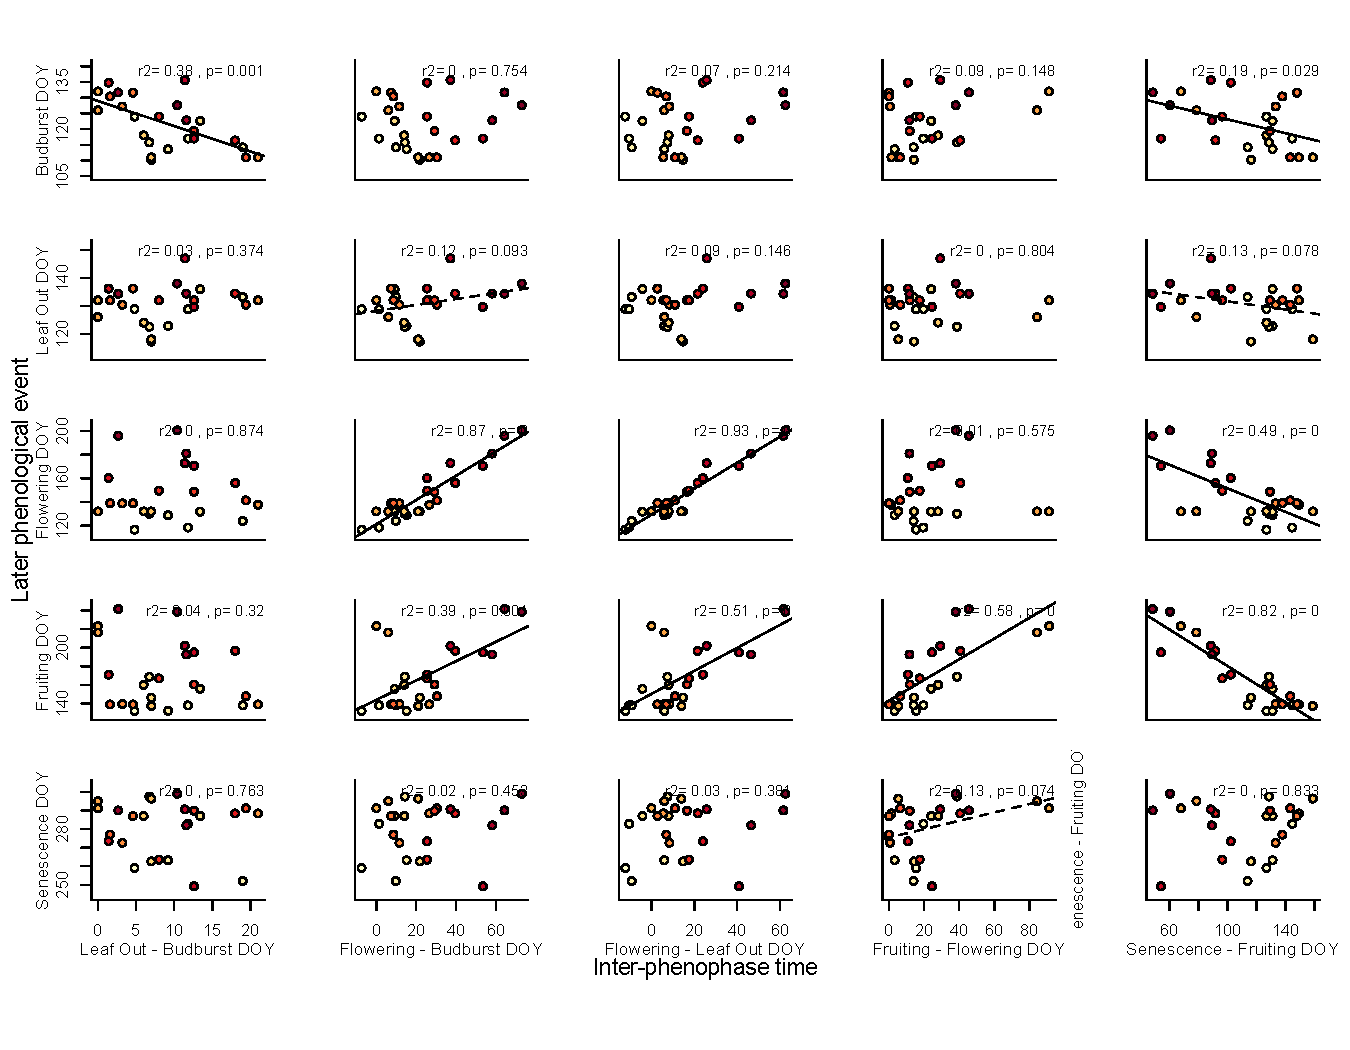
\includegraphics{../analyses/figures/adj_stagesmegaplot_col_YOR.pdf}
  \caption{\textbf{Relationships among phenological stages and inter-phenophase duration across the 25 focal species.} Inter-phenophase duration is the time between the start of the earlier phenological event and the start of the later phenological event, e.g., the number of days between the species' mean start of flowering and its mean start of fruiting. Linear models were fit with the species-level mean day of year of the later phenological stages as the response variable, and inter-phenophase duration as the explanatory variable. R\textsuperscript{2} and \textit{p}-value for each model are shown, with solid lines representing model fit when \textit{p}<0.05 and dashed lines representing model fit when 0.05<\textit{p}<0.10. Full model statistics are summarized in Table S1 in the Supplemental Materials. Species are color-coded as in Figure 3.}
  \label{fig:inter}
   \end{figure}


%%%%%%%%%%%%%%%%%%%%%%%%%%%%%%%%%%%%%%%%
\end{document}
%%%%%%%%%%%%%%%%%%%%%%%%%%%%%%%%%%%%%%%%
